\section{eplusssz.\textless{}ext\textgreater{}}\label{eplusssz.ext}

This file is the result of the system sizing calculation. As usual, the file can be read into a spreadsheet for easy viewing. System Sizing (see Sizing:System object) performs a special calculation that, to oversimplify, sums up the results of the zone sizing calculation and saves the results in the system sizing arrays for reporting on component size requirements.

An excerpt of the file:

Time,:Des Heat Mass Flow {[}kg/s{]},:Des Cool Mass Flow {[}kg/s{]},:Des Heat Cap {[}W{]},:Des Sens Cool Cap {[}W{]},

00:15:00,1.063942E+00,0.000000E+00,5.944201E+03,0.000000E+00,

00:30:00,1.063942E+00,0.000000E+00,5.944201E+03,0.000000E+00,

00:45:00,1.063942E+00,0.000000E+00,5.944201E+03,0.000000E+00,

01:00:00,1.063942E+00,0.000000E+00,5.944201E+03,0.000000E+00,

01:15:00,1.063942E+00,0.000000E+00,5.944200E+03,0.000000E+00,

01:30:00,1.063942E+00,0.000000E+00,5.944200E+03,0.000000E+00,

01:45:00,1.063942E+00,0.000000E+00,5.944200E+03,0.000000E+00,

02:00:00,1.063942E+00,0.000000E+00,5.944200E+03,0.000000E+00,

02:15:00,1.063942E+00,0.000000E+00,5.944200E+03,0.000000E+00,

02:30:00,1.063942E+00,0.000000E+00,5.944200E+03,0.000000E+00,

02:45:00,1.063942E+00,0.000000E+00,5.944200E+03,0.000000E+00,

03:00:00,1.063942E+00,0.000000E+00,5.944200E+03,0.000000E+00,

03:15:00,1.063942E+00,0.000000E+00,5.944200E+03,0.000000E+00,

03:30:00,1.063942E+00,0.000000E+00,5.944200E+03,0.000000E+00,

03:45:00,1.063942E+00,0.000000E+00,5.944200E+03,0.000000E+00,

04:00:00,1.063942E+00,0.000000E+00,5.944200E+03,0.000000E+00,

04:15:00,1.063942E+00,0.000000E+00,5.944200E+03,0.000000E+00,

04:30:00,1.063942E+00,0.000000E+00,5.944200E+03,0.000000E+00,

04:45:00,1.063942E+00,0.000000E+00,5.944200E+03,0.000000E+00,

05:00:00,1.063942E+00,0.000000E+00,5.944200E+03,0.000000E+00,

05:15:00,1.063942E+00,0.000000E+00,5.944200E+03,0.000000E+00,

05:30:00,1.063942E+00,0.000000E+00,5.944200E+03,0.000000E+00, = = = reduced for brevity = = =

Coinc Peak~~ ,1.063943E+00,1.378986E+00,5.944199E+03,2.165922E+04,

NonCoinc Peak,1.063943E+00,1.553319E+00,5.944199E+03,2.165922E+04,

\subsubsection{Field: Time}\label{field-time-20160420}

Calculation time -- this will show the time steps used by the simulation and by the sizing calculation.

\subsubsection{Field: Des Heat Mass Flow {[}kg/s{]}}\label{field-des-heat-mass-flow-kgs}

Calculated design heating mass flow rate.

\subsubsection{Field: Des Cool Mass Flow {[}kg/s{]}}\label{field-des-cool-mass-flow-kgs}

Calculated design cooling mass flow rate.

\subsubsection{Field: Des Heat Cap {[}W{]}}\label{field-des-heat-cap-w}

Calculated design heating capacity.

\subsubsection{Field: Des Sens Cool Cap {[}W{]}}\label{field-des-sens-cool-cap-w}

Calculated design sensible cooling capacity.

\subsubsection{Line: Coinc Peak}\label{line-coinc-peak}

The values in this line only apply to the Mass Flow Rates. The coincident peak cooling mass flow rate is the maximum of the sum of the zone peak cooling mass flow rates occurring at each time step. The coincident peak heating mass flow rate is the maximum of the sum of the zone peak heating mass flow rates occurring at each time step.

\subsubsection{Line: NonCoinc Peak}\label{line-noncoinc-peak}

The values in this line only apply to the Mass Flow Rates. The noncoincident peak cooling mass flow rate is the sum of the zone peak cooling mass flow rates, no matter what time of day the individual zone peaks occurred. The noncoincident peak heating mass flow rate is the sum of the zone peak heating mass flow rates, no matter what time of day the individual zone peaks occurred.

Or as depicted graphically:

\begin{figure}[hbtp] % fig 5
\centering
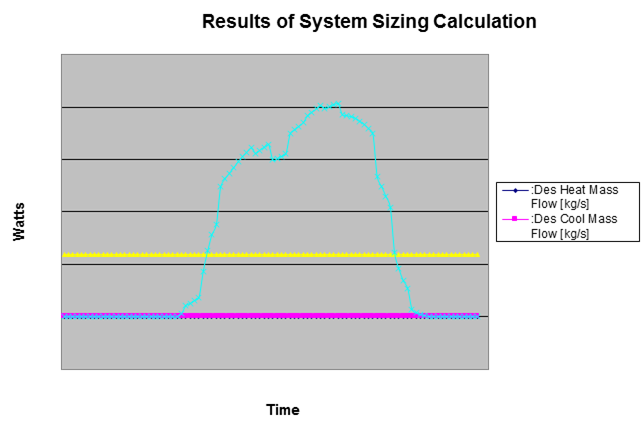
\includegraphics[width=0.9\textwidth, height=0.9\textheight, keepaspectratio=true]{media/image017.png}
\caption{System Size depiction from eplusout.ssz \protect \label{fig:system-size-depiction-from-eplusout.ssz}}
\end{figure}
